\section{Design Details}\label{sec:details}

In this section, we present the details of \concept{}. We
first give the details of decision graph, followed by the path
computation and the data path generation. 

\vspace{-2mm}
\subsection{Decision Graph}

The Decision Graph (DG) is used to capture the forwarding decisions process of
packets and stateful operations on packets. 
%capture the trace of every packet applied by the program. The trace is the decision dependencies (\ie, the results of packet fields test statements and middlebox processing statements) of a packet and its returned path (\ie, path constraints). In this paper, we focus on the waypoints constraint (\ie, a sequence of nodes in the network that packets should pass through) as it would complicate the path computation involving the stateful middleboxes. 
We define a DG as a directed acyclic graph (with a single root) that has three types of nodes: packet-test nodes, middlebox-operation nodes, and action nodes (mapping to three basic primitives, packet-test, middlebox, and route algebra). The first two nodes are the internal nodes of DG while the last one is the leaf node. An out-edge of a node can specify a range of packets (if the node is a packet-test node) or a result from a middlebox (if the node is a middlebox-operation node). For example, the DG of the motivating program is shown in Fig.~\ref{fig:dg-example}. Note that we do not focus on the computation of DG from a program which can be achieved by existing (compiler) work~\cite{arashloo2016snap}~\cite{smolka2015fast}.

\begin{figure}[!htbp]
%\vspace{-2mm}
\centering
\begin{subfigure}{0.8\linewidth}
      \centering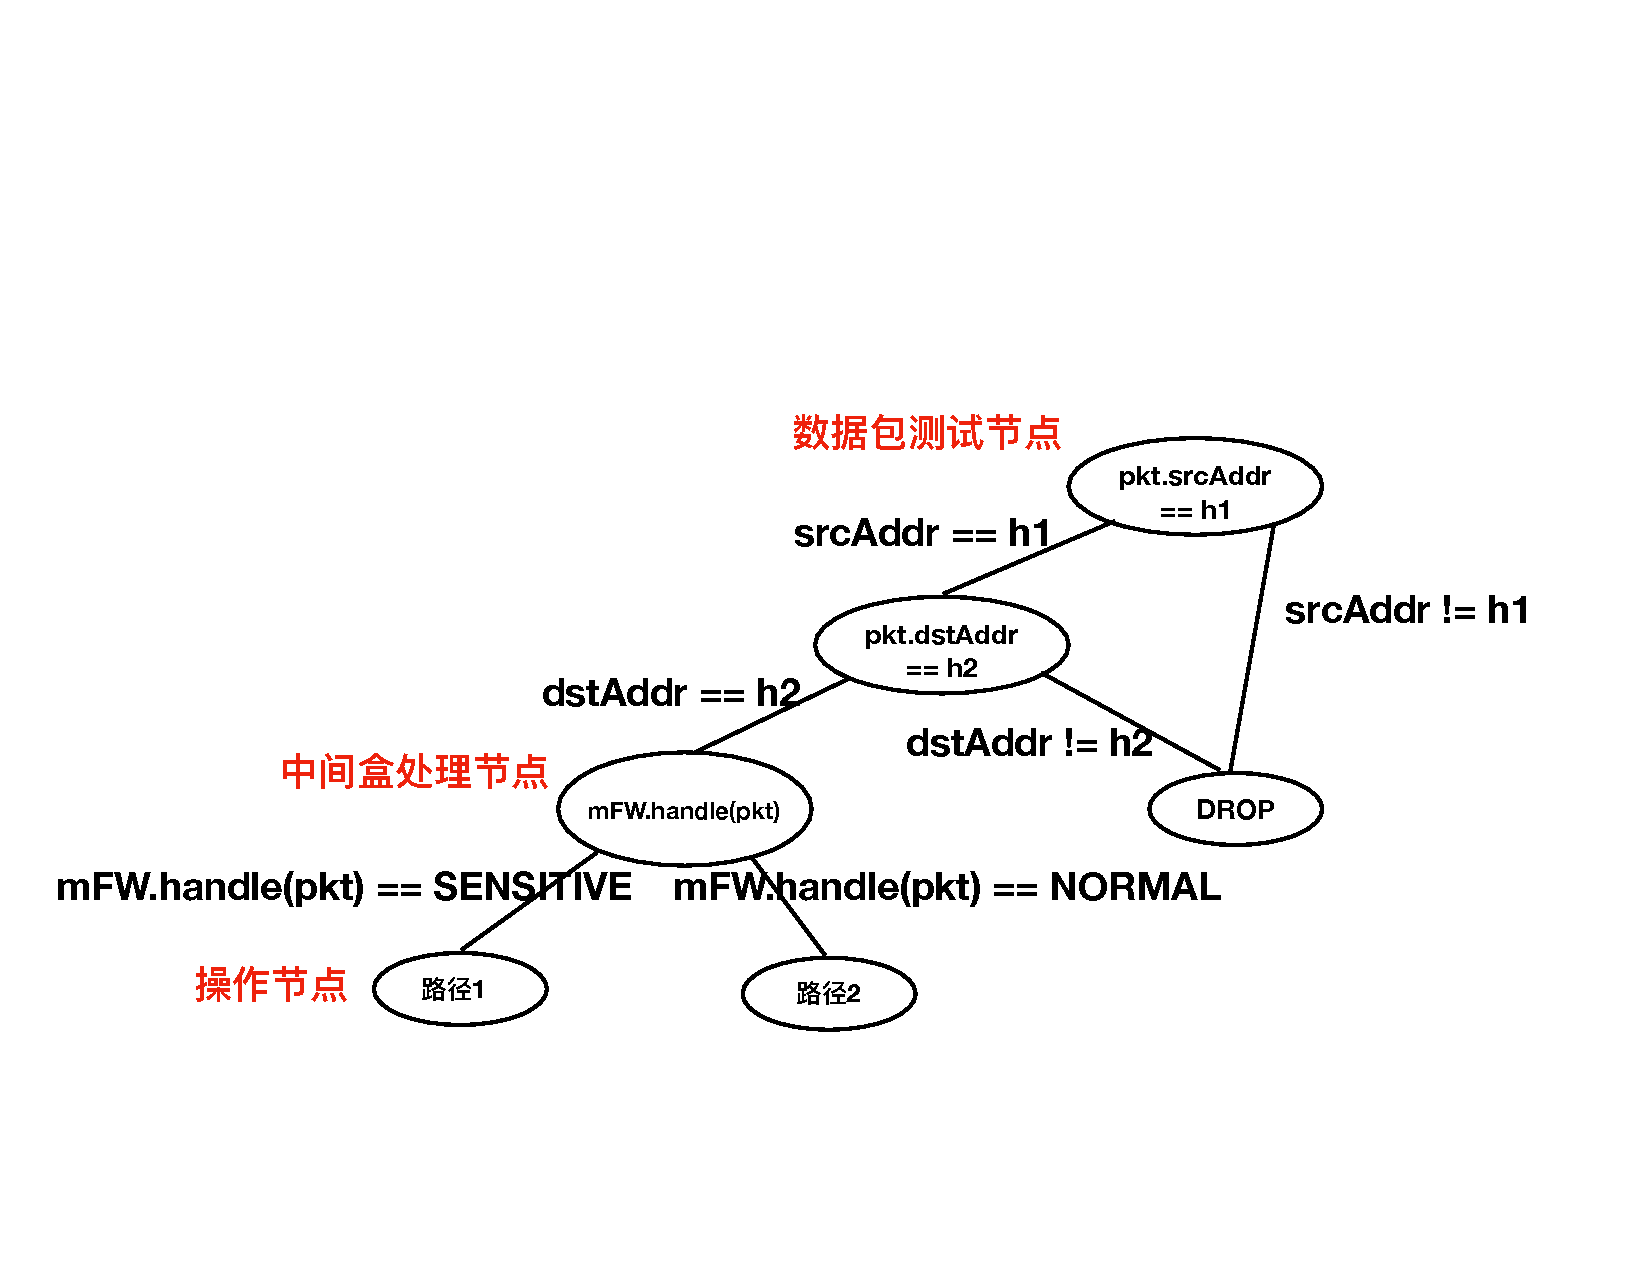
\includegraphics[width=\linewidth]{figures/ss-126.pdf}
\end{subfigure}
\vspace{-2mm}
\caption{\small Example of DG.}
%\vspace{-2mm}
\label{fig:dg-example}
\end{figure}

Given a DG, we denote the sequence of nodes and edges from the root to an action node (\ie, path constraint $pc$) as the trace of $pc$ ($T(pc)$). Then, given a trace $T(pc)$, we denote the middlebox-operation nodes of $T(pc)$ as $M(pc)$ (\ie, a sequence of nodes). As middlebox-operation nodes represent the packet handling of middleboxes, to not form loops, every middlebox-operation node can only appear once in $M(pc)$. Also, by extracting middlebox-operation nodes that represent stateful middleboxes from $M(pc)$, we have a subsequence of $M(pc)$ that every node is for stateful middlebox operations (denoted by $M^s(pc)$). Given a $T(pc)$, the SPC for its action node can be easily computed as the $T(pc)$ gives the trace of the packet enters the action node.

\vspace{-2mm}
\subsection{Path Computation}

As the leaf nodes in DG are path constraints, path computation targets to compute the concrete paths for these leaf nodes with a system performance objective. (And if leaves are concrete paths, the path computation just skips them.)

\para{Packet forwarding model}: Before path computation, we first give a packet forwarding model with DG in the network as the following. As shown in Fig.~\ref{fig:pfm-example}, given a path ($gw, a, b$) in the motivating example, logically we consider every switch in the path has the DG of the example program where $P$ indicates a packet-test node, $M$ indicates a middlebox-operation node, and $A$ indicates an action node. The $A$ node with red color represents the corresponding constraints for the path. The first packet of the flow (arriving at $gw$) starts to traverse the DG as the red line in the figure. When the packet meets a middlebox-operation node, it will be sent to the corresponding middlebox through the tunnel. After the processing, the middlebox will send the packet back and share its local state (\ie, by installing/modifying rules in the state table) for the flow with the corresponding middlebox-operation nodes (each node can be viewed as a pair of state table and match table) at switches along the path. (If the middlebox is stateful, then it does not set any state but makes the packet carry the state.) After the traversal of the DG (\ie, arriving at the leaf node along the red line), the packet will get the path and should be forwarded along the path. As local states have been shared with corresponding middlebox-operation nodes (or carried by the packet for stateful middleboxes) at other switches, the packet does not need to be sent to the middlebox again at the next switch. We denote a forwarding of a packet as stable forwarding if the packet does not access any stateless middlebox (compared with the first packet that should access them). Based on the stable forwarding, we can extend original SPC variable to \codeword{SPC.stable} which means the system path constraints only for stable forwarding paths (\ie, remove the stateless middleboxes). Then, to allow the state sharing, \codeword{SPC.stable} should be used as \codeword{SPC} includes the whole constraints for all packets including the first packet that must pass through all the middleboxes.

\begin{figure}[!htbp]
%\vspace{-2mm}
\centering
\begin{subfigure}{0.8\linewidth}
      \centering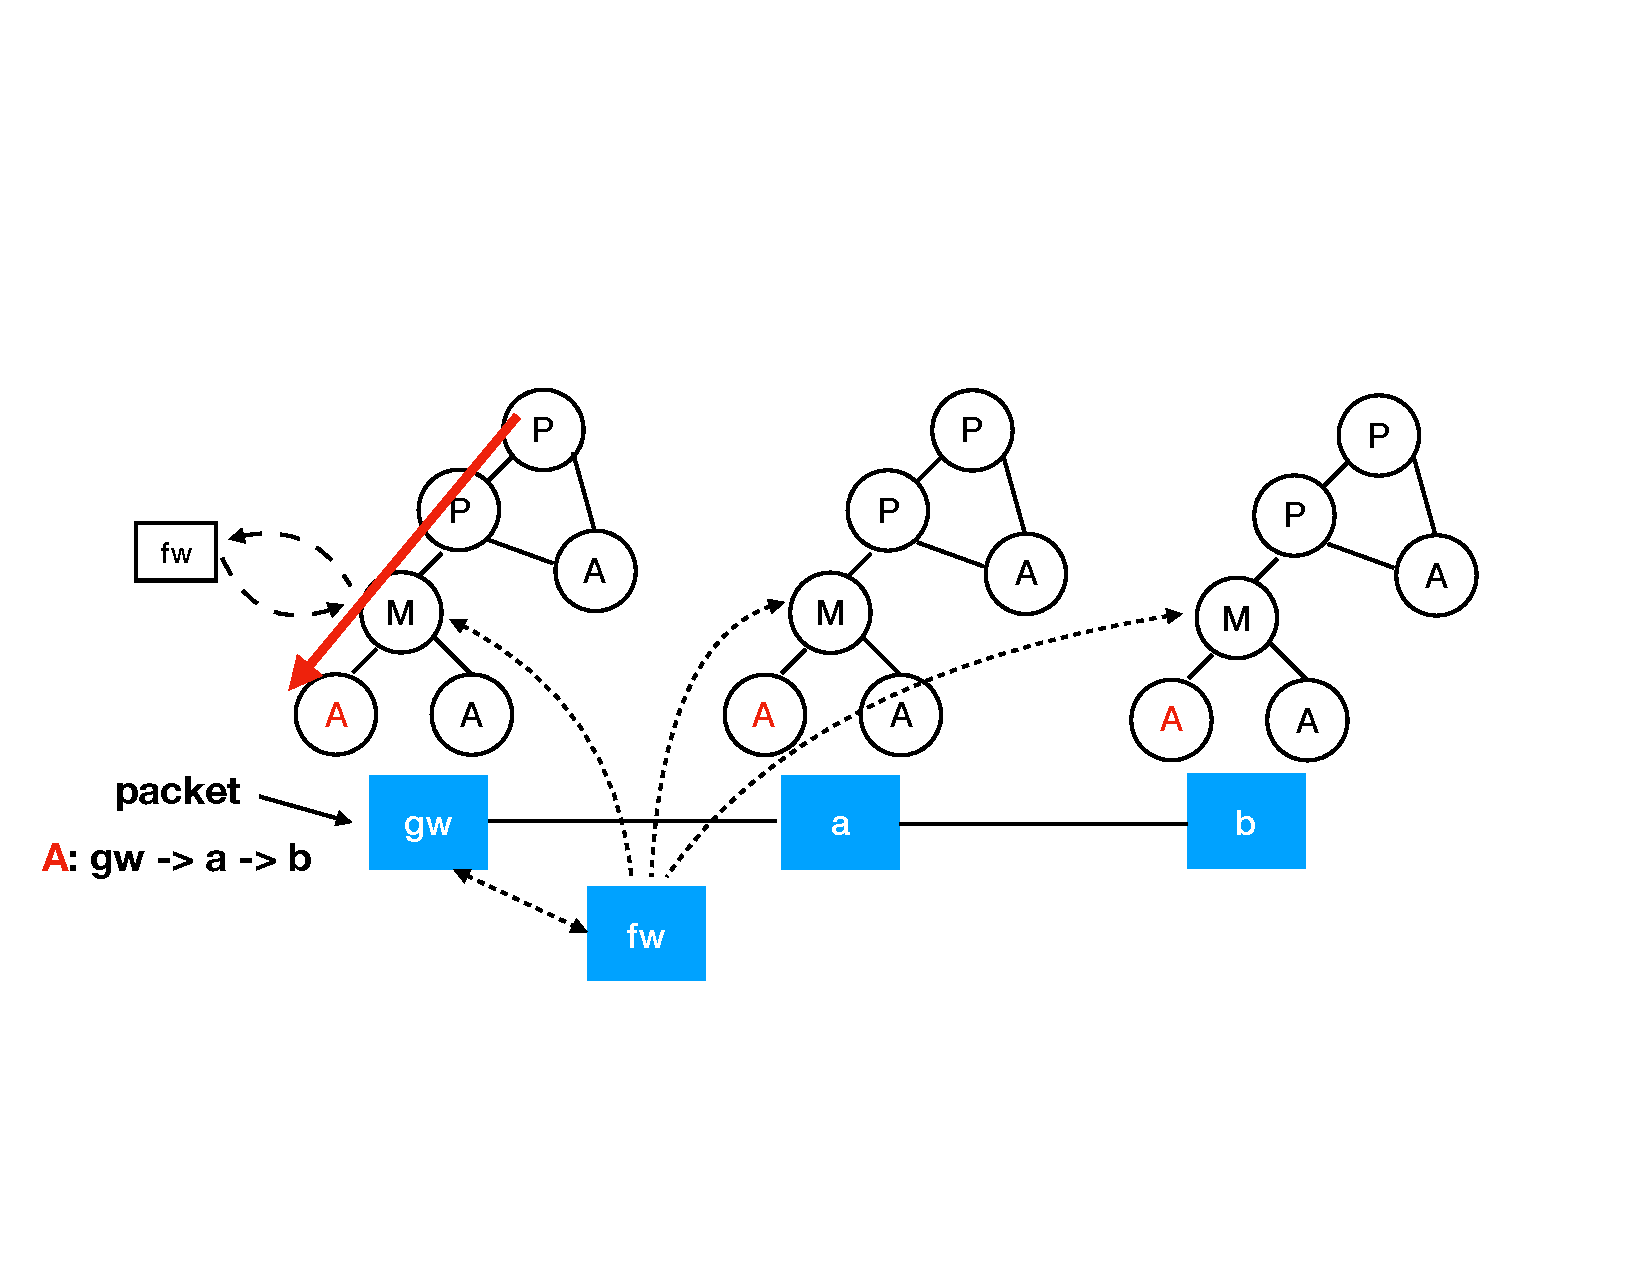
\includegraphics[width=\linewidth]{figures/ss-127.pdf}
\end{subfigure}
\vspace{-2mm}
\caption{\small Packet forwarding model with DG.}
%\vspace{-2mm}
\label{fig:pfm-example}
\end{figure}

%We denote the forwarding of the packets do not involve the stateless middleboxes as the stable forwarding.

%\para{Initialization for waypoints constraints}: As the initial process, for every action node in the DG, system should identify its source and destination nodes in the network. (This can be achieved by the hints from network operators as~\cite{arashloo2016snap}.) Then, add the source and destination nodes and also the $M^s(pc)$ to the corresponding waypoints constraint as the processing of stateful middleboxes should have a correct order. We consider the waypoints constraint as a set of node pairs where a pair has the form $(x, y)$ which indicates packets must pass through $x$ before $y$. (Note that $x$ and $y$ can be source/destination nodes.)

\para{System objective}: Based on the model, as the forwarding of the first few packets has little influence on the performance of the flow, a simple path computation (that only considers the stable forwarding) would be the following. We consider the objective of the network is to maximize the total throughput, \ie, maximize $\sum_ib_i$ where $i$ is the index of the path constraint $pc_i$ and $b_i$ is its throughput. The definition of variables can be found at Table~\ref{table:variables}. And the constraints can be found at Table~\ref{table:constraints} (where $Path(x, y, E)$ means there exists a simple path starting from $x$ to $y$ in $E$). In this paper we focus on the waypoints constraints for the path constraints (as they may complicate the path computation) and we consider the waypoints constraint as a set of node pairs where a pair has the form $(x, y)$ which indicates packets must pass through $x$ before $y$. (Note that $x$ and $y$ can be source/destination nodes.)

\begin{table}[]
\scriptsize
\begin{tabular}{l|l}
Variable     & Description                                                             \\ \hline
$u_i$, $v_i$ & The source and destination nodes of path constraint $pc_i$                            \\ 
$E$          & All edges (an edge $e$: $(e.src, e.dst)$) in the network                       \\
$m_e$        & The maximum bandwidth of $e$                                            \\
$W_i$        & A set of node pairs of $pc_i$ \\
$z^i_e$      & The edge $e$ is selected by $pc_i$ \\
$b_i$          & The bandwidth of flows using the path for $pc_i$                                   
\end{tabular}
\caption{\small Notation.}
\label{table:variables}
\end{table}

\begin{table}[]
\scriptsize
\begin{tabular}{l|l}
Constraint                                        & Description                               \\ \hline
$\forall i, \forall (x, y) \in W_i, Path(x, y, E)$                    & Path constraints                  \\
$\forall i, Path(u_i, v_i, E)$      & Path exists in $E$     \\
$\forall e \in E, \sum_ib_i*z^i_e \le m_e$   & Bandwidth constraints for edges
\end{tabular}
\caption{\small Constraints.}
\label{table:constraints}
\end{table}

As the system path constraints have been added into the path constraints (by using the \codeword{SPC.stable}), the correctness can be guaranteed. And it enforces a packet must get results of stateful middleboxes and then select the correct path.

%However, this simple solution can get optimal paths only if all the middleboxes are stateless. If there is a stateful middlebox, the constraints of stable forwarding should not only consider the waypoints constraints specified by the program as it also must pass through the stateful middleboxes.
%
%Then, people may add another constraint as the following: $\forall (x, y) \in M^s(pc_i), Path(x, y, E)$. This constraint enforces that the optimal paths must pass through all the stateful middleboxes in a correct order (\ie, $M^s(pc_i)$). This seems correct as now the stable forwarding includes the stateful middleboxes. 
%
%However, this is not enough. Considering the example as shown in Fig.~\ref{fig:c-example}. As the middlebox $M$ is stateful, the new added constraint enforces that the computed optimal paths should pass through $M$. However, the result could be that $M$ is behind the branch of waypoints $b$ and $c$. In this case, when a packet arrives at $a$, it cannot decide how to forward to $M$ as which path to select depends on the result of $M$.
%
%\begin{figure}[!htbp]
%%\vspace{-2mm}
%\centering
%\begin{subfigure}{0.9\linewidth}
%      \centering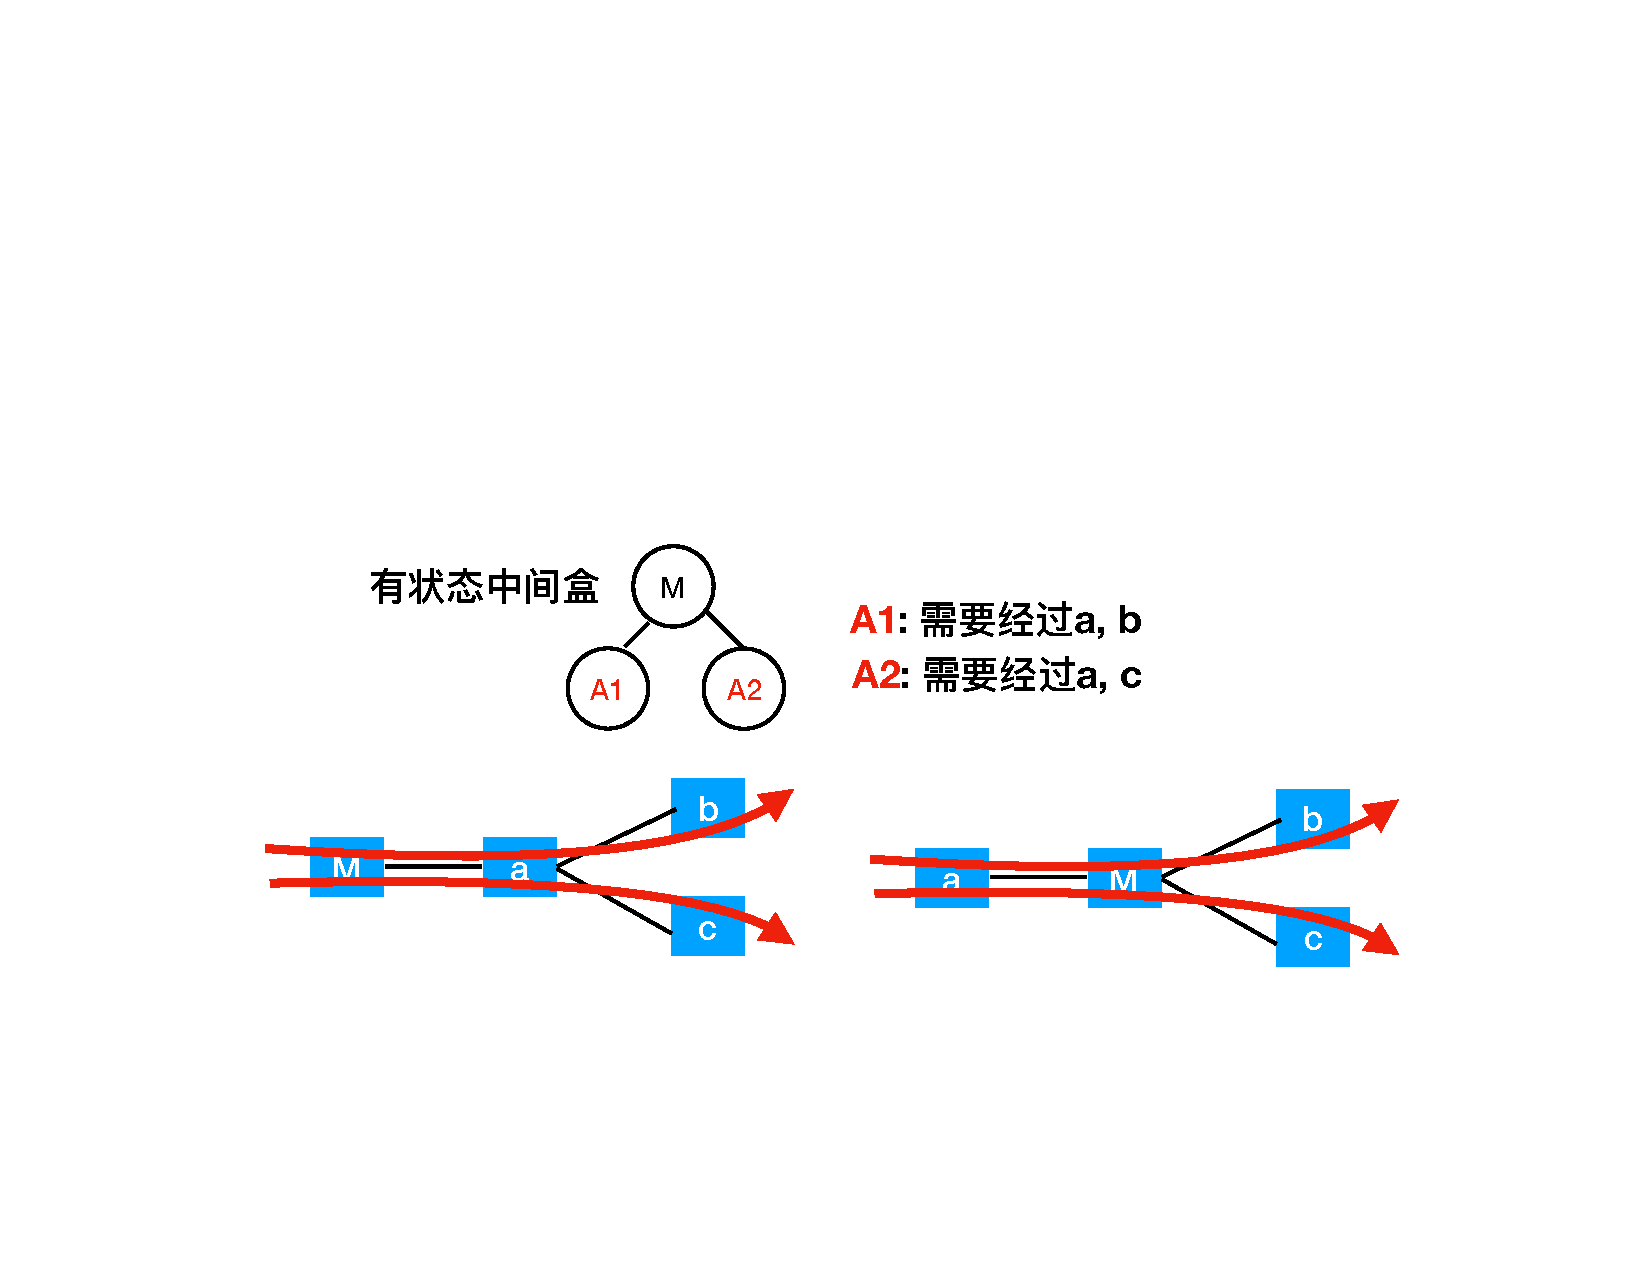
\includegraphics[width=\linewidth]{figures/ss-128.pdf}
%\end{subfigure}
%\vspace{-2mm}
%\caption{\small An example to show that the dependencies between middlebox-operation nodes and waypoints should be considered.}
%%\vspace{-2mm}
%\label{fig:c-example}
%\end{figure}
%
%To resolve the issue in Fig.~\ref{fig:c-example}, one solution is to add constraints $(M, b)$ and $(M, c)$ to  $A_1$ and $A_2$ respectively. Then the paths in Fig.~\ref{fig:c-example} cannot exist as they does not satisfy the constraints. The idea is to enforce a packet must get results of stateful middleboxes and then select the correct path.

However, the current path constraints may cause \emph{excessive constraints} for paths. For example, a stateful middlebox-operation node ($M$) has two path constraints $A_1$ and $A_2$ as its children in a DG. And, $A_1$ specifies a path must pass through switches $s_1, s_2$; $A_2$ specifies a path must pass through switches $s_1, s_3$. Then, the path constraints have $(M, s_1)$ for both $A_1$ and $A_2$ as it simply connects the waypoints constraint in \codeword{SPC.stable} and $s_1, s_2$ (also $s_1, s_3$). However, this is only a sufficient condition as some other conforming paths are excluded (\eg, $s_1 \rightarrow M \rightarrow s_2\ (s_3)$).

\para{Waypoints constraints computation}: Instead of simply connecting two waypoints constraints, now we give an algorithm to compute the waypoints constraints that enforces all the paths are correct and no conforming paths can be excluded. The high-level structure of the algorithm is to do a depth-first traversal for a DG. The traversal only considers the stateful middlebox-operation nodes and action nodes (and traverses a stateful middle operation node only after all its children are finished). When traversing a stateful middlebox-operation node, we can get all possible waypoints constraints under its decision. Then, the processing of the node is to update these constraints (each of which can be modeled as a directed acyclic graph, DAG). As discussed before, we do not want to add excessive constraints. And the solution is simple: When processing a middlebox node $M$, if all the no-incoming-edge nodes of $M$'s possible constraints (\ie, DAGs) are the same, then skip these nodes recursively until these nodes are not the same and then add edges ($M$, $x$) to each of DAGs where $x$ is the node of the location that the skipping process stopped at. The insight is that, skipping a node is safe if and only if the node is the next waypoint node for \emph{all} the possible paths. For the example in Fig.~\ref{fig:skip}, the node $M$ has four possible path constraints (DAGs) and $a$ should be skipped when updating them.

\begin{figure}[!htbp]
%\vspace{-2mm}
\centering
\begin{subfigure}{0.8\linewidth}
      \centering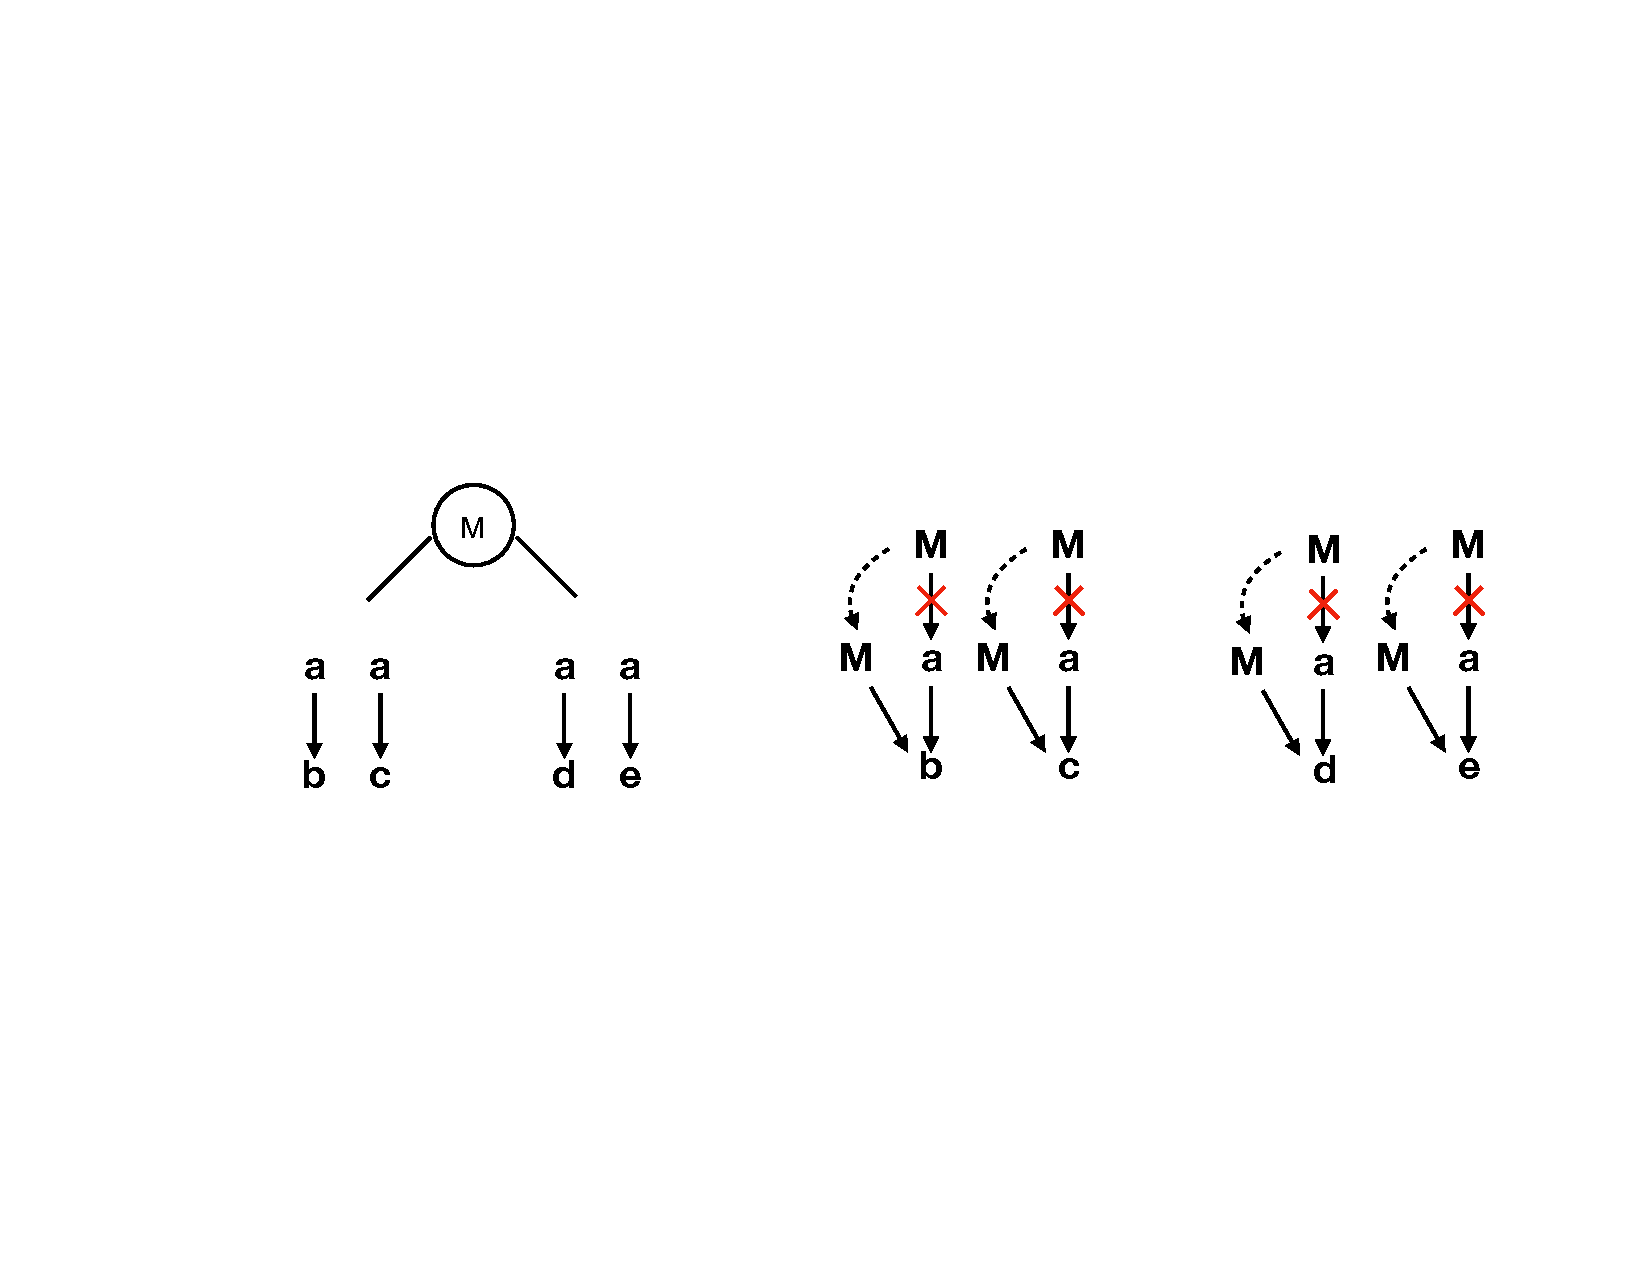
\includegraphics[width=\linewidth]{figures/ss-129.pdf}
\end{subfigure}
\vspace{-2mm}
\caption{\small Skip the same nodes.}
%\vspace{-1mm}
\label{fig:skip}
\end{figure}



%
%Based on the idea, we give an algorithm to solve the issue for general cases. The high-level   
%
%
%First, given a middlebox operation node $m$ in a DG, we denote a set of topology ordered waypoints constraints that $m$ can reach to in DG as $R(m)$. Also $R(m)$ can be partitioned by the out-edges of $m$, \ie, the out-edge $m^o_i$ has a subset of $R(m)$ (denoted by $R^i(m)$). If there is a stateful middlebox node $n$ in $R^i(m)$ that $m \rightarrow n \in M^s(p_i)$, then add $m \rightarrow n$ to $R^i(m)$. Given the new $R^i(m)$, we denote a set of nodes in $R^i(m)$ that has no order with $m$ as free nodes with $m$ in $R^i(m)$. Then, we extract the subgraph from $R^i(m)$ that only includes these free nodes into a new graph: $Free(R^i(m))$. Then, for all the $Free(R^i(m))$, if there exists $Free(R^i(m))$ is not equal to $Free(R^j(m))$, it means the result of $m$ is required to choose which out-edge to go. Therefore, the following constraints are need. For all the $Free(R^i(m))$, skip the same no-incoming-edge nodes recursively until it does not exist, and add the constraints: $m \rightarrow nexts(Free(R^i(m)))$ where $nexts(Free(R^i(m)))$ is the set of no-incoming-edge nodes after the skipping. Finally, for all stateful middlebox operation nodes, do the previous processing. For example, for the DG in Figure 6 (XXX), $M_2$ adds new constraints: $M_2 \rightarrow b$ and $M_2 \rightarrow c$ for $A_1$ and $A_2$. (Similar for $M_3$.) And then $M_1$ adds $M_1 \rightarrow M_2 (M_3)$.

\vspace{-2mm}
\subsection{Datapath Generation}

\para{Remove redundant nodes of DG}: After the path computation, there are concrete paths for all the leaf nodes in DG. We follow the packet forwarding model described previously that all the switches in the network have the same DG. It is easy to observe that if a switch does not belong to a path, then the corresponding leaf node of the path can be removed (and then the no-out-edge internal nodes). Also, by converting the path in a leaf node to the next hop in the network, we may still remove redundant nodes. Still consider the firewall example. After we convert the paths to next hops, we find that the two leaf nodes of the middlebox node are the same, \ie, switch $a$ in the network. This means the middlebox-operation node has no meaning for the gateway $gw$ since whatever the result of the node is, the next hop does not change. Therefore, we can remove the node and replace with the leaf node with the next hop $a$. Fig.~\ref{fig:rv} illustrates the process. 

Then, for the switch side, based on the updated DG, it can generate tables and flow rules easily with the multi-table pipeline structure. Note that a middlebox-operation node can be viewed as a state table following a match table. As for the middlebox side, if it is a stateless middlebox, then for the datapath it only needs to care about is switch-middlebox tunnels which also can be easily generated. For the stateful middleboxes, as they belong to computed paths, they can be viewed as switch nodes with stateful functions that can embed the results to the packets. When a packet meets a stateful middlebox node in DG of a switch, and the node cannot be replaced with a leaf node, then any next hop under the node is acceptable since it must eventually arrive at the middlebox and any path from the switch to the middlebox must follow the path constraints.

\begin{figure}[!htbp]
%\vspace{-2mm}
\centering
\begin{subfigure}{0.8\linewidth}
      \centering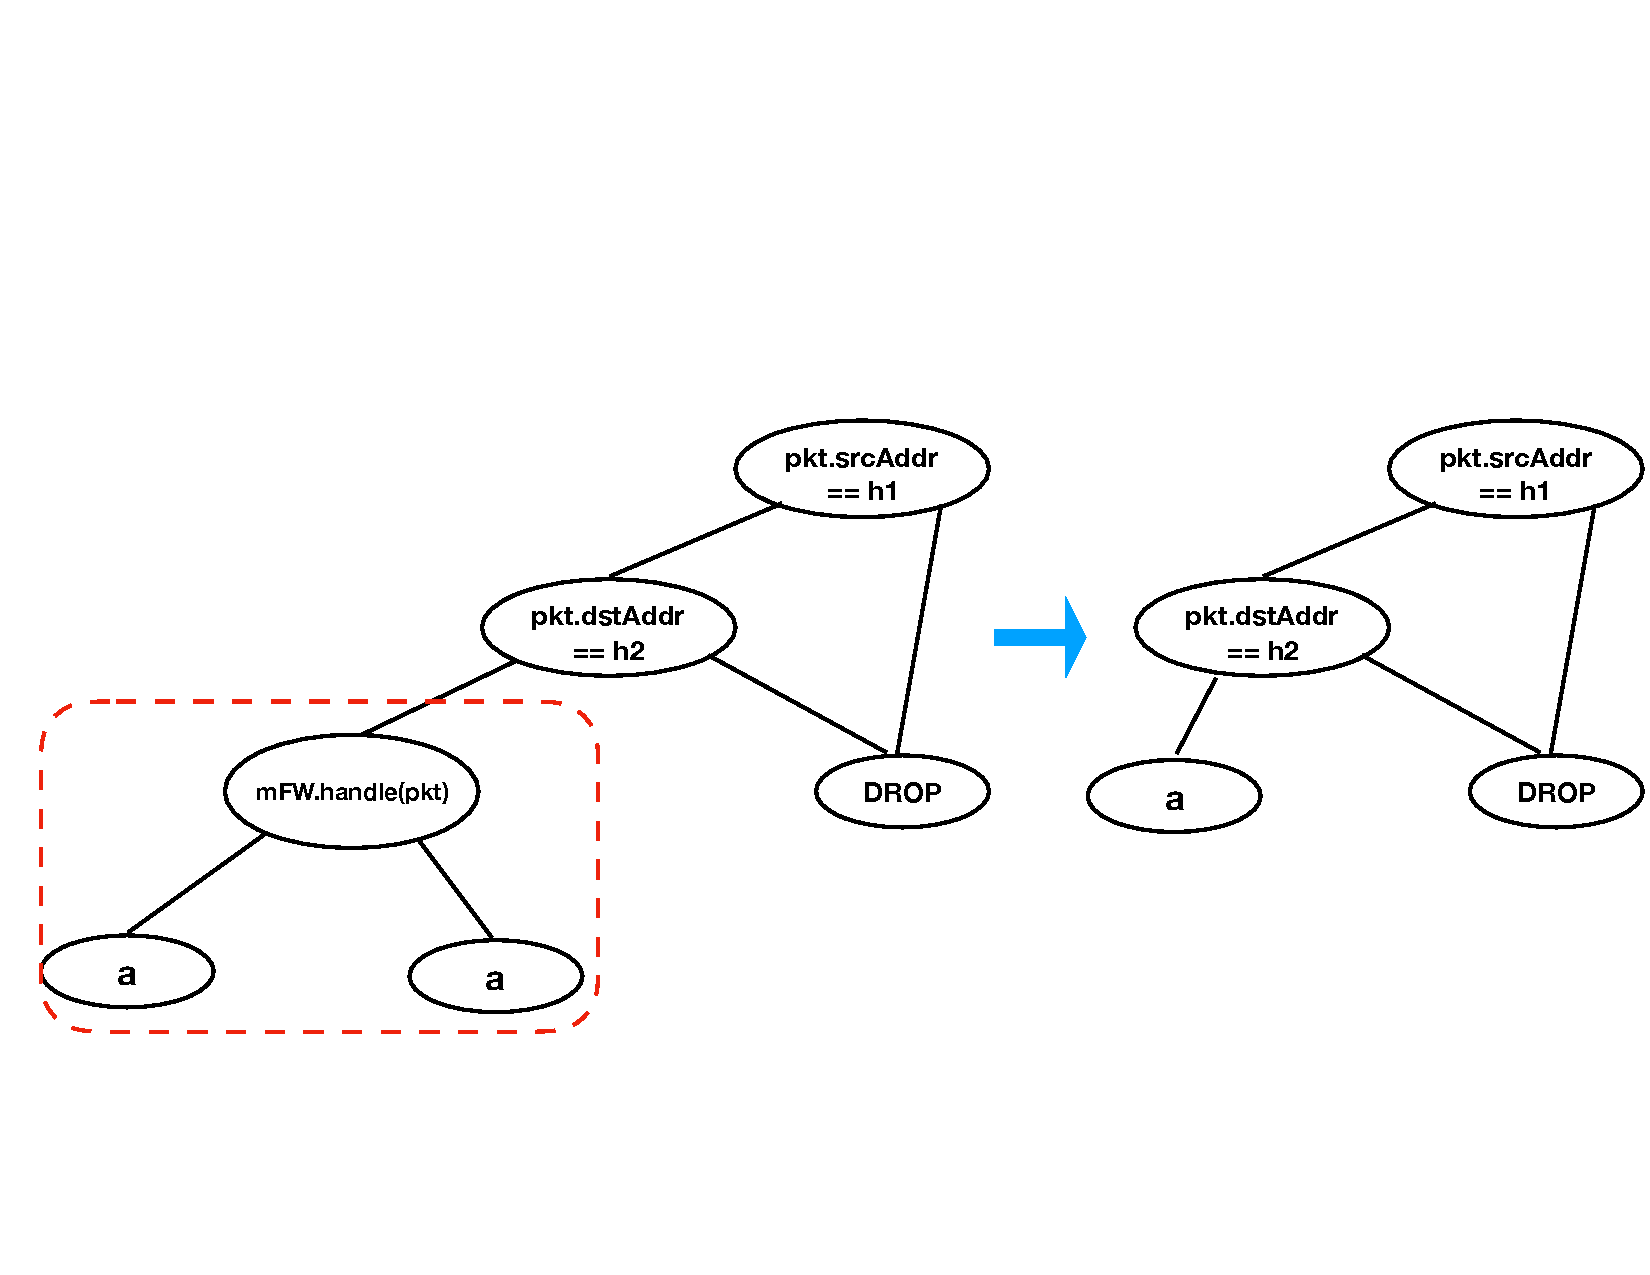
\includegraphics[width=\linewidth]{figures/ss-130.pdf}
\end{subfigure}
\vspace{-2mm}
\caption{\small Remove redundant middlebox nodes.}
%\vspace{-2mm}
\label{fig:rv}
\end{figure}

\para{Order of messages}: The next issue is how a stateless middlebox share local states (\ie, update states) in other switches. It needs to guarantee that for any targeting switch, the update message should arrive earlier than the packet. For example, in the firewall example, only the step 2 is finished, step 3 can be executed. Then a simple solution can be making the packet carry the update message. Different with the state carrying for stateful middleboxes, this message can install/modify rules in the state table of the corresponding middlebox-operation node.





%In this section, we will discuss the implementation of the general network-wide stateful packet processing to provide a more flexible state updates. First, we will show the consistency problem in the general network-wide stateful packet processing. Then, we will present two techniques for the problem.
%
%\subsection{Consistency problem}
%
%As discussed in Sec. 2, the consistency requirement demands a packet must see the newest states which may be updated by the previous packet. Let us consider the example shown in Figure. 3 with two switches $sw_1$ and $sw_2$ and two maps $m_a$ and $m_b$ are stored in the two switches respectively. Now a flow with packets $pkt_1, pkt_2, ..., pkt_i, ...$ try to be processed with three operations: read $m_a$; read $m_b$; write $m_a$. Then, the problem arises that when $pkt_i$ tries to read $m_a$, how to guarantee that $pkt_i$ reads the updated value of $m_a$?
%
%%figure 3
%\begin{figure}[!htbp]
%%\vspace{-2mm}
%\centering
%\begin{subfigure}{0.7\linewidth}
%      \centering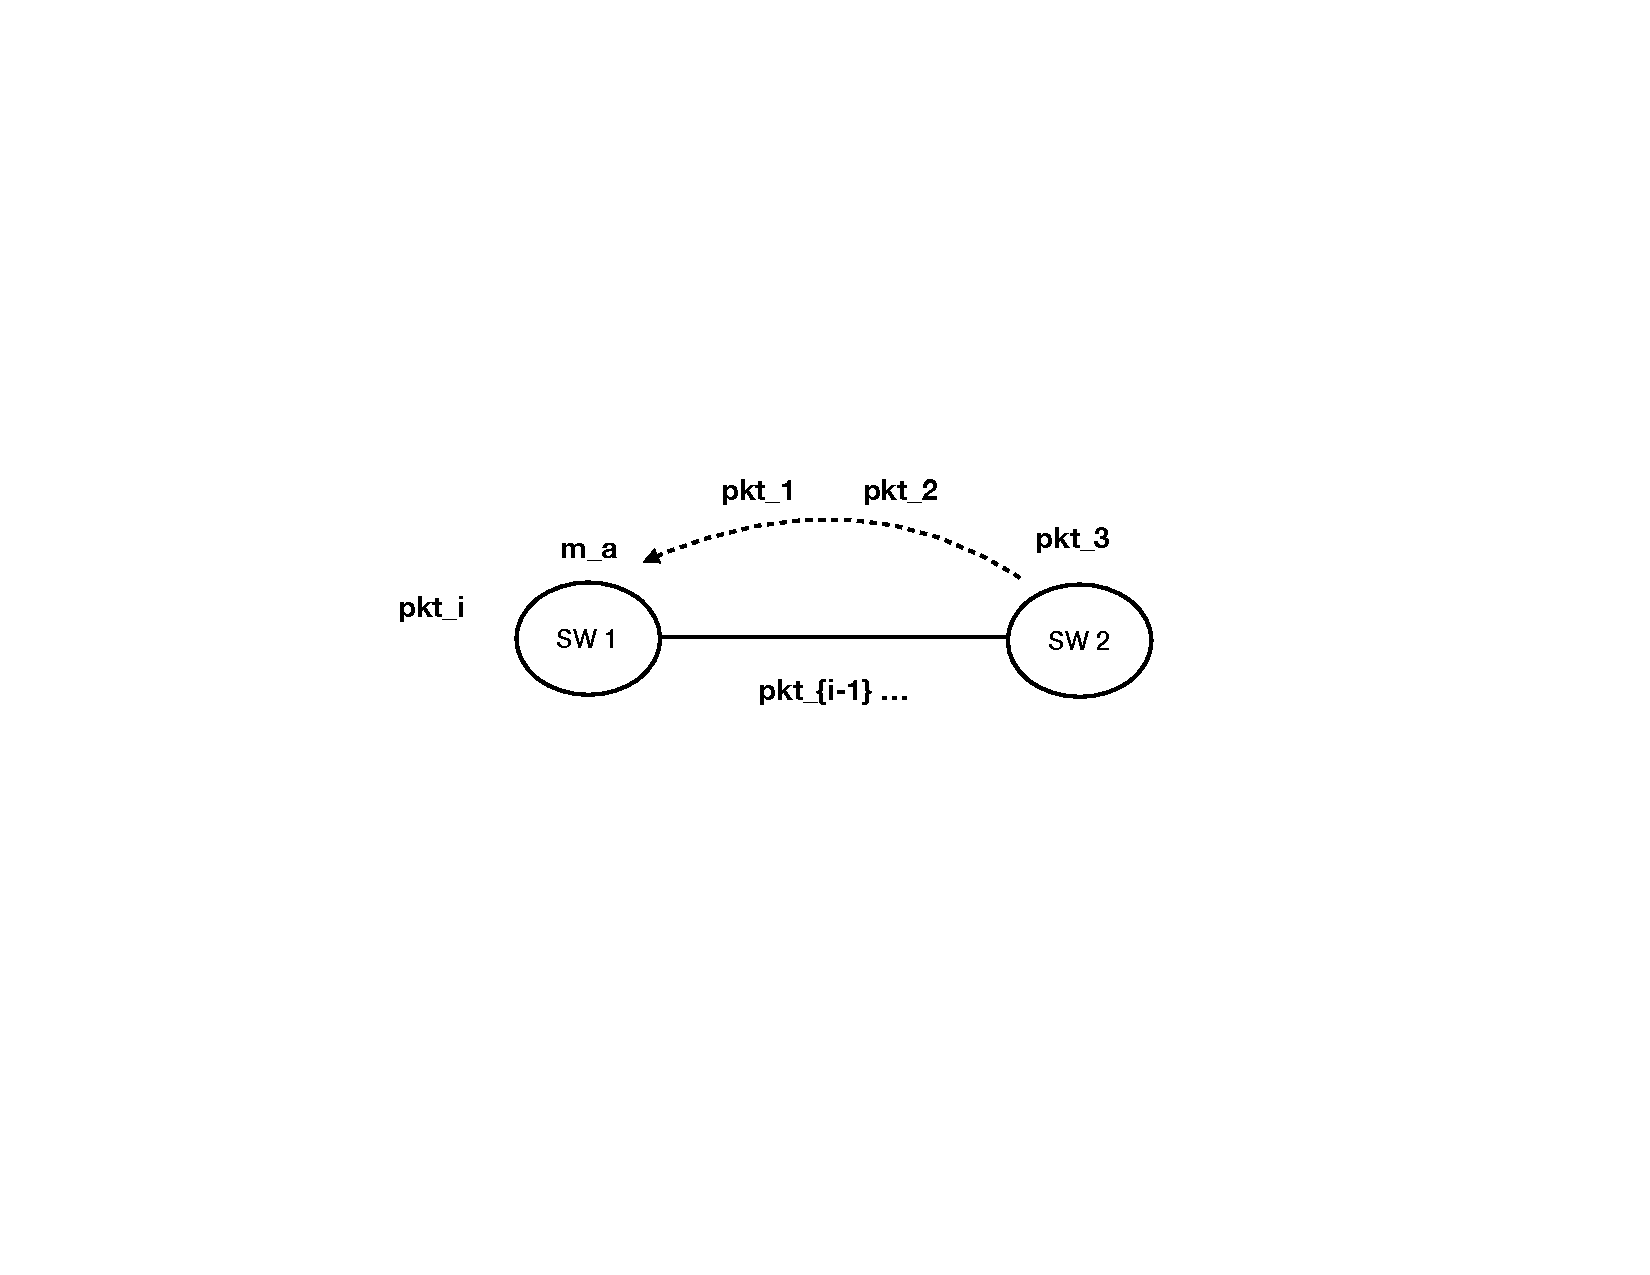
\includegraphics[width=\linewidth]{figures/69.pdf}
%\end{subfigure}
%%\vspace{-2mm}
%%\caption{\footnotesize{The CDF of job latency local and remote jobs.}}
%\caption{\small Example of two switches.}
%%\vspace{-2mm}
%\label{fig:mtv-example}
%\end{figure}
%
%A naive solution to the problem is to let every packet wait until the previous packet has updated the state. But there are two issues: one is how the packet knows the state has been updated (the previous packet may not update the state); two is that the waiting packets in the switch not only causes the latency issue but only occupies the queue storage in the switch. In the following subsections, we will show two techniques to solve the problem.
%
%\subsection{Fixed-route packets}
%
%Consider the Figure 3, when $pkt_i$ arrives at $sw_1$ trying to access $m_a$, the first thing $pkt_i$ needs to check is that whether there are previous packets trying to update $m_a$. As the waiting approach may cause serious performance issue, a new design is needed.
%
%As the constraint that there is only one loop for a flow to access a state variable (discussed in the target paragraph), if there are any packets (in the same flow with $pkt_i$) trying to update $m_a$, these packets should be in the loop. Then, if $pkt_i$ can pass through the loop (without causing any updates to any state), when $pkt_i$ arrives $sw_1$ again, it can make sure that all the previous packets (if any) have finished the updates. This can be achieved by adding a special tag (Fixed-Route, FR) to $pkt_i$. When $pkt_i$ tries to access $m_a$, $pkt_i$ should first be tagged with $FR_a$ specifying the packet $pkt_i$ is trying to access $m_a$. Then, the FR $pkt_i$ is forwarded to the corresponding loop of $m_k$. When $pkt_i$ with the FR tag arrives at $sw_1$ after passing through the loop, it should first remove the FR tag from $pkt_i$ and then $pkt_i$ can access $m_a$ with any operations.
%
%\begin{figure}[!htbp]
%%\vspace{-2mm}
%\centering
%\begin{subfigure}{0.7\linewidth}
%      \centering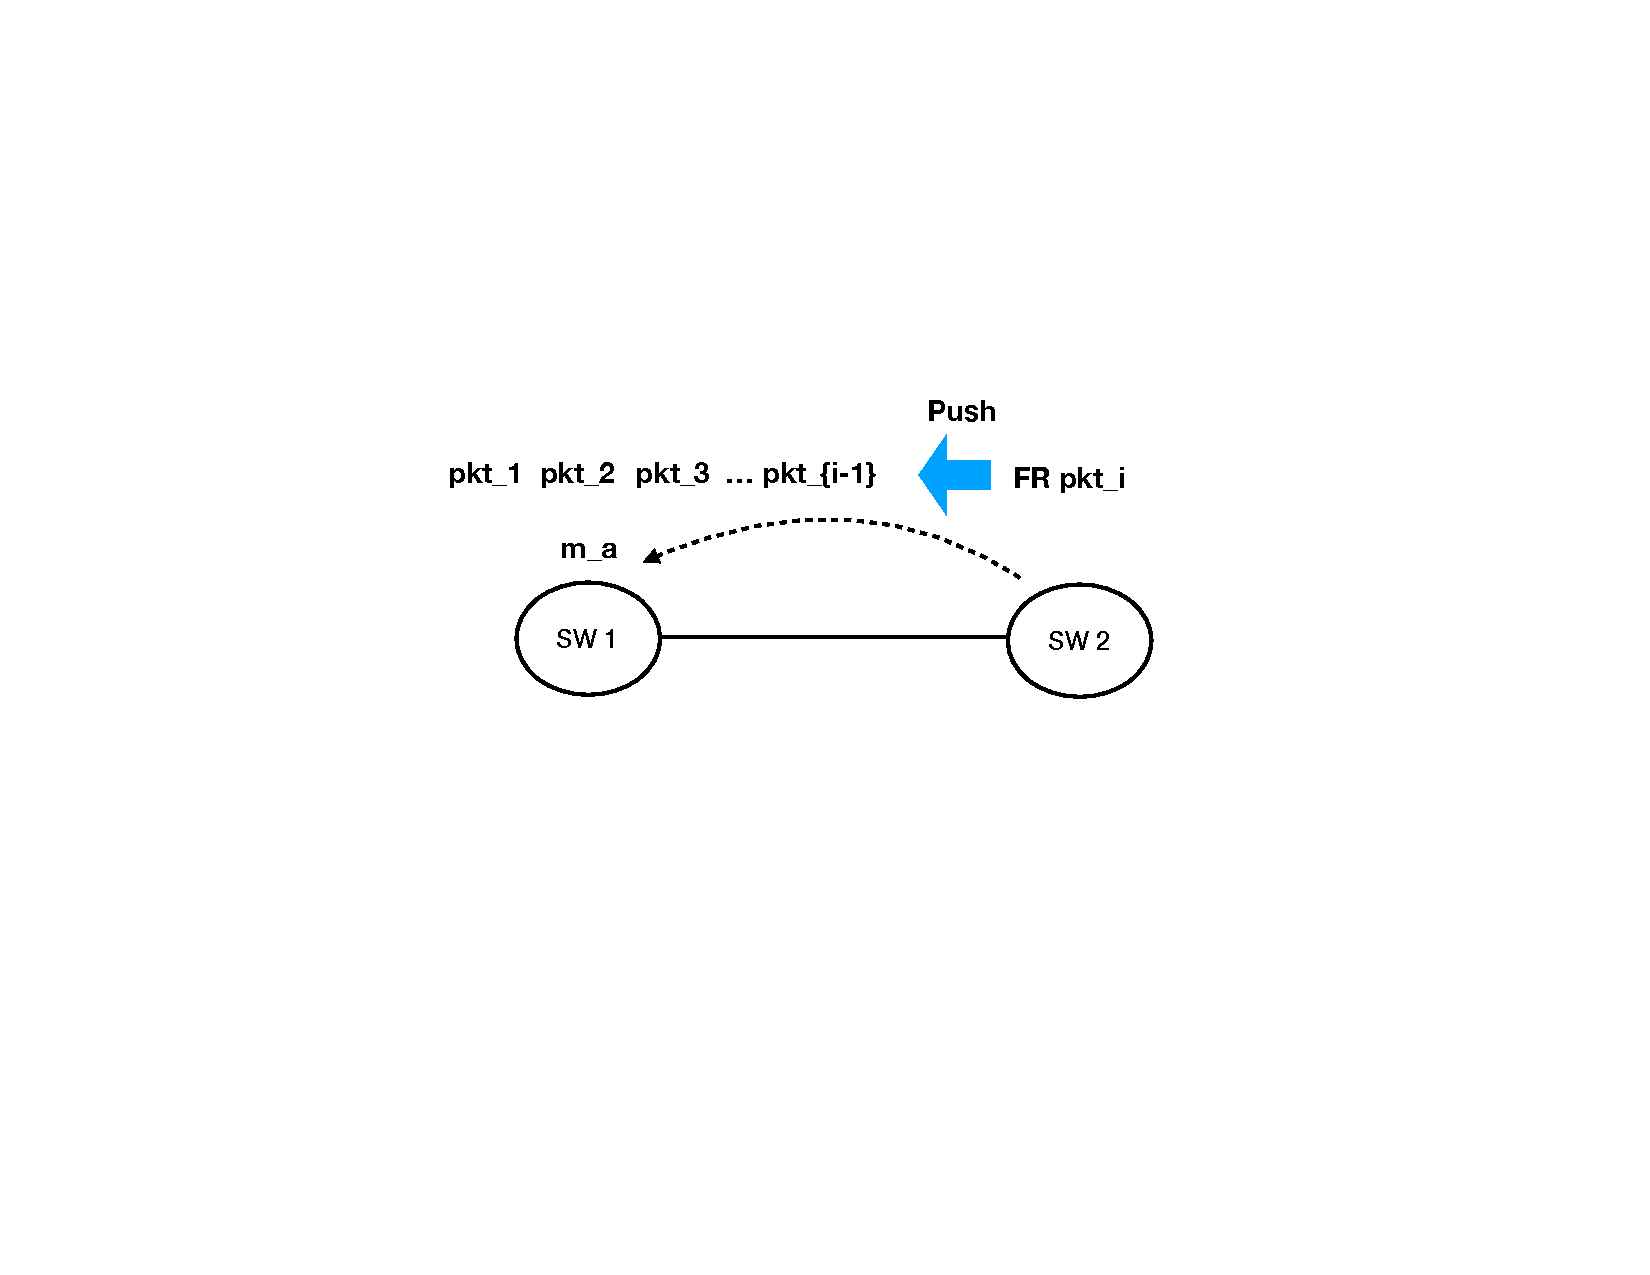
\includegraphics[width=\linewidth]{figures/70.pdf}
%\end{subfigure}
%%\vspace{-2mm}
%%\caption{\footnotesize{The CDF of job latency local and remote jobs.}}
%\caption{\small Example of FR packets push the previous packets.}
%%\vspace{-2mm}
%\label{fig:mtv-example}
%\end{figure}
%
%The intuition is that the FR packet will ``push out'' all the potential previous packets that may update $m_a$ in the loop.Therefore, whenever the FR packet arrives $sw_1$, it can make sure that all the previous updates have been applied. However, one issue of the FR tag design is that it seems \emph{all} packets should experience the loop which may cause potential latency.
%
%%
%%
%%\subsection{Two-version states}
%%
%%First, to not let packets wait in the switch, a simple solution is to forward packets. As the consistency requirement is for packets belong to the same flow with the same path (TODO), if no state updated, a packet should follow the same path as the previous packet does. Now the problem is how to make the packet see the updated state.
%%
%%The solution is to maintain two versions of states: one is for the new incoming packets; the other is for the packets arriving twice. Specifically, given a state $m_k$ stored in switch $sw_k$, we maintain two versions of $m_k^{old}$ and $m_k^{new}$. In the beginning, $m_k^{old}$ keeps the original value of $m_k$ and $m_k^{new}$ is null. When a new incoming packet $pkt_i$ arriving at $sw_k$ tries to read $m_k$, as this is the first time $pkt_i$ reads $m_k$, the result is the value of $m_k^{old}$. Over a period of time, $pkt_i$ arrives $sw_k$ again and tries to write a value to $m_k$. Then, the updated value is stored in $m_k^{new}$. Now consider another packet $pkt_{i+1}$ following $pkt_i$ arrives at $sw_k$. Packet $pkt_{i+1}$ tries to read $m_k$ and it returns the value of $m_k^{old}$ which leads $pkt_{i+1}$ to follow the same path of $pkt_i$. When $pkt_{i+1}$ arrives at $sw_k$ again, it realizes that the value of $m_k$ has been updated (as the value is not null), then it reads the updated value from $m_k^{new}$. At this point, it achieves that $pkt_{i+1}$ sees the updated value of $m_k$. Table XXX shows which version of $m_k$ should be considered with different cases. Note that first arrival means that the packets is the new incoming and second arrival means that it is the second time the packet arrives at $sw_k$.
%%
%%\begin{table}[]
%%\begin{tabular}{|l|l|l|l|l|}
%%\hline
%%\multirow{2}{*}{} & \multicolumn{2}{l|}{$m_k^{new}$ == null} & \multicolumn{2}{l|}{$m_k^{new}$ != null} \\ \cline{2-5} 
%%                  & Read from           & Write to           & Read from           & Write to           \\ \hline
%%First arrival                & $m_k^{old}$         & $m_k^{old}$        & $m_k^{old}$         & $m_k^{old}$        \\ \hline
%%Second arrival                & $m_k^{old}$         & $m_k^{new}$        & $m_k^{new}$         & $m_k^{new}$        \\ \hline
%%\end{tabular}
%%\end{table}
%%
%%To make a packet knows that whether it is the second time to arrive at a switch and try to access (including read/write) a state variable at the switch, a simple but useful approach is to embed the historical accesses of state variables to the packet. When a packet tries to access a state variable, it first needs to check the historical accesses of state variables to see whether the state variable has been accessed before. After the checking, it can decide which version of the state should be read from/written to.
%%
%%The insight of the two-version design is that whenever a packet arrives a switch and tries to access a state, it can realize two things: one is that whether this is the first arrival or the second arrival; two is that whether the state has been updated or not. If it is the second arrival and the state has been updated, then for the consistency requirement, the packet must be processed as if it is the \textbf{first} time the packet tries to access the state. (Note that in this case, the exceeding part of the historical accesses of state variables also should be deleted.) Then, the consistency is guaranteed as the packet has seen the updated state.
%%
%%\subsection{Multi-version states}
%%
%
%
%\subsection{Counter and timer to break loop}
%
%The issue of the FR tag design is that a packet \emph{always} first be tagged with FR and pass through the loop, and then the packet can be processed with normal operations. In this section, we will show how to use a counter and a timer to break the loop easily.
%
%%the old version of a state even the state has been updated, which may cause a ``redundant'' loop of state accesses that increases the latency.
%
%For each state variable $m_k$, it has a counter $c_k$ to record the current number of FR packets (with $FR_k$) in the corresponding loop of $m_k$ that try to update $m_k$. Specifically, when a packet is tagged with $FR_k$, the counter $c_k$ increases one to indicate there is a new packet entering $m_k$'s corresponding loop. When a FR packet with $FR_k$ finish the loop and arrive the switch of $m_k$, the counter $c_k$ decreases one to indicate there is a packet removed from the loop. Then, the counter $c_k$ is able to give the current number of packets in the loop.
%
%As the TCP packets enter the network in a burst way (for UDP packets, as there is no order among them, the consistency requirement is not important), if the interval time between two bursts of packets is large enough, the packets in the loop can be all pushed out indicated by the value of counter equals to zero. Fortunately, as the burstiness of TCP is at RTT and subRTT scale [ref: XXX], and the loop latency in data planes should be much smaller than that [ref: XXX], for every first packet of bursts of packets trying to access $m_k$, the counter $c_k$ has a high possibility to be zero.
% 
%When the counter of $m_k$ becomes zero, any packet can access $m_k$ immediately without tagged with $FR_k$ as there is no packet in the loop trying to update $m_k$. However, when a packet accesses $m_k$, the packet can either access $m_k$ or not, which cannot be determined. Therefore, it cannot make sure whether the packet is in the loop or not.
%
%Here we introduce a timer $t_k$ for $m_k$. The timer $t_k$ records the time of the last packet without FR tag that accesses $m_k$ and leaves the switch. When a new packet arriving at the switch and trying to access $m_k$, if the counter $c_k$ is zero, then compute the time: $current\_time - t_k$. If the computed time is larger than the time $t_x$ where $t_x$ is larger than the latency time of the corresponding loop of $m_k$, it is very likely that the previous packet does not enter the loop. Then, the new packet can access $m_k$ and leaves the switch (also update the value of the timer $t_k$). As the loop is fixed, by choosing the value of $t_x$, the error rate can be reduced to packet loss rate. Also the computation of the latency of the corresponding loop of $m_k$ can be easily achieved as it can sample several FR packets passing through the loop and compute the average latency for these FR packets. However, if the computed time is smaller than the time $t_x$, then the packet should be tagged with FR and forwarded to the loop which has been discussed in previous subsection.
%
%%
%%A naive solution to break the loop is that when the state is updated (\ie, the new version of the state is not null), the packet accesses the new version of the state. However, this solution is wrong: the new version of the state can be updated multiple times. It cannot guarantee that all the previous updates have been applied to the state when a packet try to access the state.
%%
%%The solution to that issue is to set a timer to a state to record the time that the last packet accesses the old version of the state. Specifically, given a state $m_k$ at switch $sw_k$, a timer $t_k$ is set to record the time that last packet $pkt_i$ access $m_k^{old}$. We denote that time as $t_k^i$. When another packet $pkt_{i+1}$ arrives at the switch and tries to access $m_k$, we compute the following interval time: $current\_time - t_k^i$. If the interval time is larger than a time $t_x$ where $t_x$ is larger than the time from $pkt_i$ sent from $sw_k$ to $pkt_i$ received again at $sw_k$ (denote as the loop time of $m_k$, \ie, LT($m_k$)), then $pkt_{i+1}$ can access the new version of $m_k$, which breaks the loop. As the state variables are already placed on the switches as well as the paths of packet processing, the computation of LT($m_k$) can be easily achieved by sending a prove packet along the corresponding path (a loop) to record the traveling time of the prove packet.
%%
%%The insight of the timer design is that if the interval time is larger than the $t_x$, then it very likely means 
%%
%
%\subsection{Multiple flows}
%
%As we have shown how to handle packets in the same flow, now let us consider the case with multiple flows. As the packets among different flows do not have any consistency requirement (this is because there is no order among packets in different flows), the single flow case can easily be extended to the multi-flow case. Given a state variable $m_k$, and flows $F_1, F_2, ..., F_n$, if $F_i$ can apply the \emph{one-loop} sequence of state operations for $m_k$, then $m_k$ should have maintain the corresponding tag $FR_k^i$, counter $c_k^i$ and timer $t_k^i$ for $F_i$. Packets in $F_i$ only need to pay attention to its own $FR_k^i$, $c_k^i$ and $t_k^i$ without involving the others.
%
%\subsection{Workflow}
%
%After discussed all the techniques, here we will show the workflow that how a packet reads/writeds states with the consistency requirement guaranteed. As shown in Figure 5, the incoming packets arriving at a stateful switches can be divided into two classes: FR tagged or not. Step 1: If a packet without FR tag arriving at a stateful switch, after matching some flow tables, it goes to the list of state variables. Step 2: Based on the flow of the packet and which state variable it tries to access, it can get the corresponding counter and timer. Step 3: After the computation for the counter and timer, the decision is made that whether the packet should be tagged with FR and forwarded, or the packet can access the required state variable. Step 4: If a packet with FR tag arriving at a stateful switch, it should go to Step 5. Step 5: First, remove the FR tag and then the packet can access required state variable.
%
%Note that how to operate with state variables (\ie, read or write) should be specified in the flow tables including matching state variables or write operations defined in the flow table actions, which is not the focus of this work.
%
%\begin{figure}[!htbp]
%%\vspace{-2mm}
%\begin{subfigure}{0.9\linewidth}
%      \centering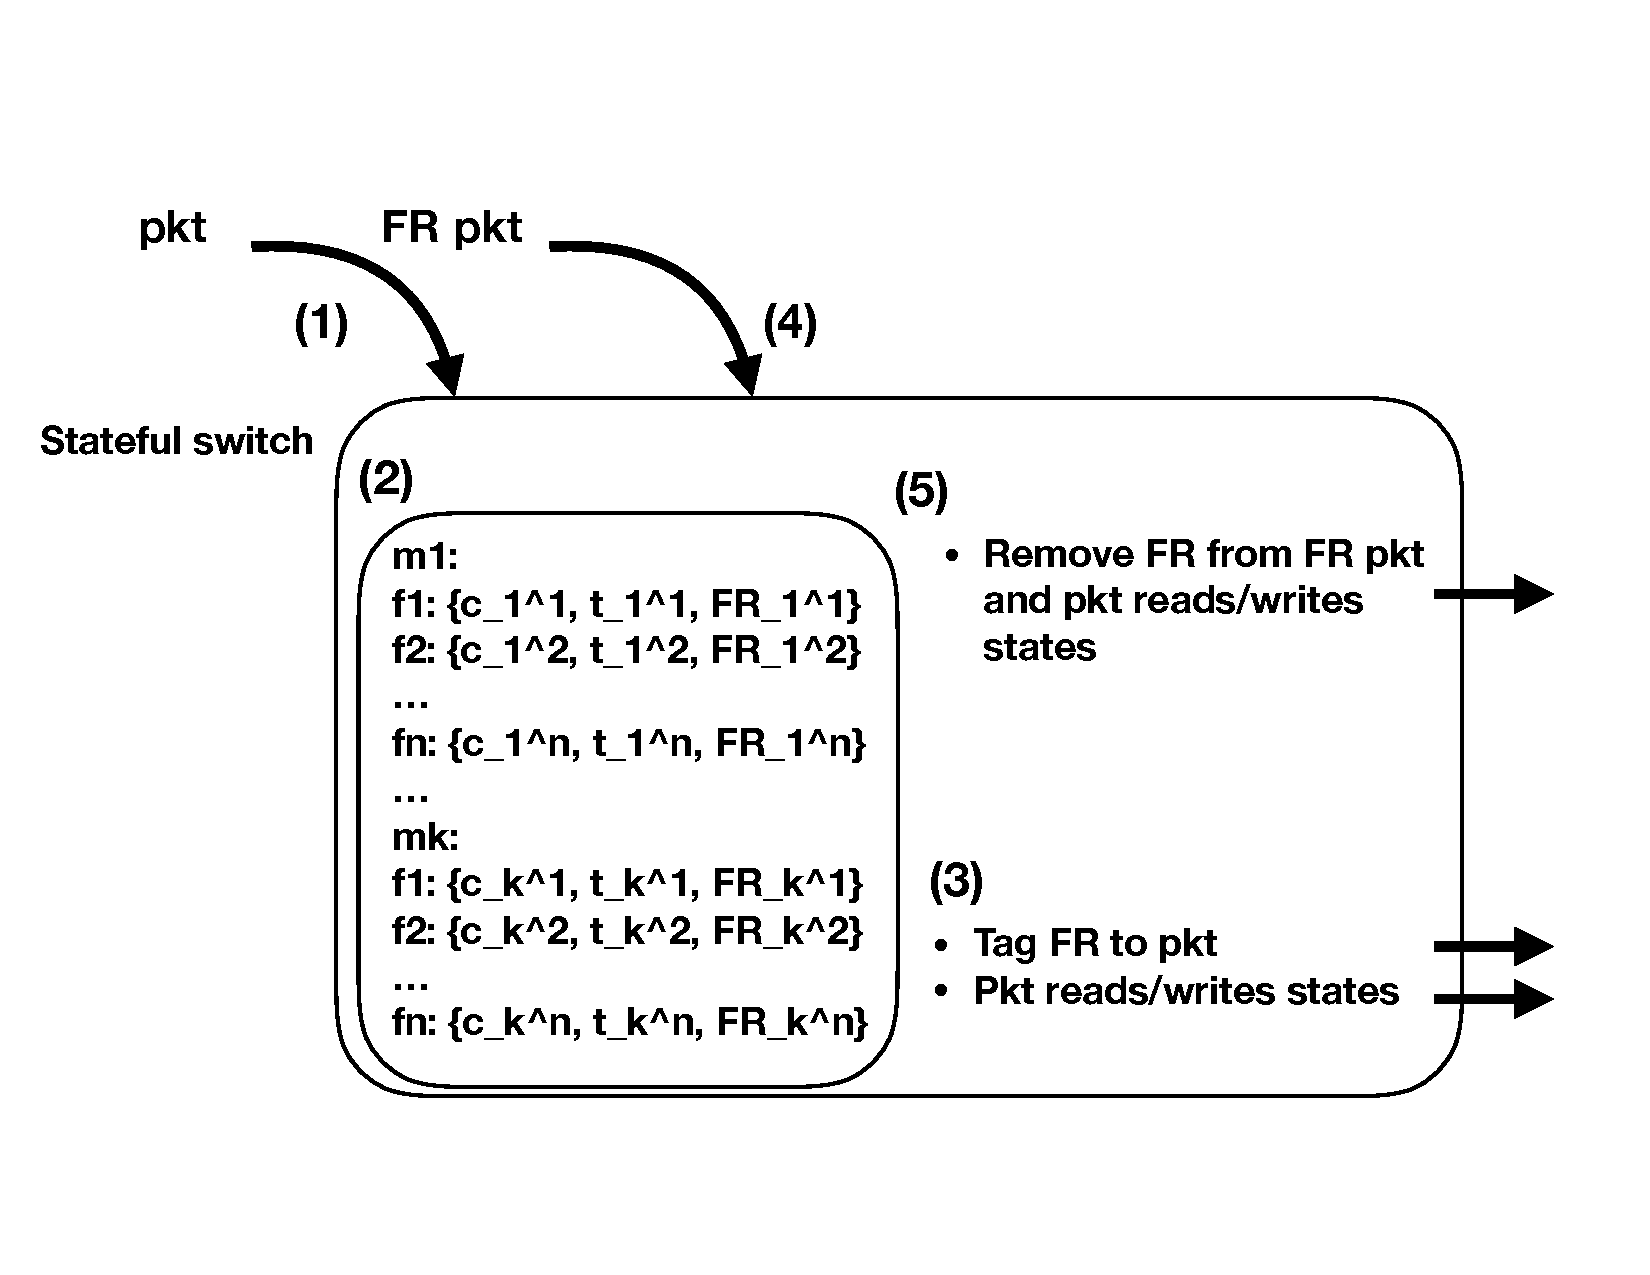
\includegraphics[width=\linewidth]{figures/71.pdf}
%\end{subfigure}
%%\vspace{-2mm}
%%\caption{\footnotesize{The CDF of job latency local and remote jobs.}}
%\caption{\small Workflow.}
%%\vspace{-2mm}
%\label{fig:mtv-example}
%\end{figure}
%
%
%
